\documentclass[aspectratio=169]{beamer}
\usetheme{Madrid}
\usecolortheme{default}

\usepackage{graphicx}
\usepackage{booktabs}
\usepackage{amsmath}
\usepackage{amssymb}
\usepackage{tikz}
\usetikzlibrary{shapes,arrows,positioning,calc,shapes.symbols,decorations.pathreplacing,shadows.blur}
\usepackage{pgfplots}
\pgfplotsset{compat=newest}
\usepackage{listings}
\usepackage{xcolor}
\usepackage[normalem]{ulem} % For \sout strikethrough

%===============================================================================
% UNIFIED BLUE COLOR PALETTE (Matching progress_slides.tex style)
%===============================================================================
% Simple color scheme: Blue for primary, Gray for neutral, Green for success only
% No custom HTML colors - use standard LaTeX xcolor mixing for consistency

%===============================================================================
% BEAMER THEME CUSTOMIZATION (Clean, minimal)
%===============================================================================
\setbeamercolor{structure}{fg=blue!70!black}
\setbeamercolor{frametitle}{fg=white,bg=blue!70!black}
\setbeamercolor{title}{fg=blue!70!black}
\setbeamercolor{subtitle}{fg=gray!60}
\setbeamercolor{author}{fg=gray!70!black}
\setbeamercolor{institute}{fg=gray!60}
\setbeamercolor{date}{fg=gray!60}
\setbeamercolor{block title}{fg=white,bg=blue!60}
\setbeamercolor{block body}{fg=gray!70!black,bg=blue!15}
\setbeamercolor{block title alerted}{fg=white,bg=blue!50}
\setbeamercolor{block body alerted}{fg=gray!70!black,bg=blue!15}
\setbeamercolor{block title example}{fg=white,bg=green!50!black}
\setbeamercolor{block body example}{fg=gray!70!black,bg=green!10}
\setbeamercolor{item}{fg=blue!60}
\setbeamercolor{itemize item}{fg=blue!60}
\setbeamercolor{itemize subitem}{fg=gray!60}
\setbeamercolor{footline}{fg=gray!60,bg=gray!10}

% Clean fonts
\setbeamerfont{title}{size=\Large,series=\bfseries}
\setbeamerfont{frametitle}{size=\large,series=\bfseries}
\setbeamerfont{block title}{size=\normalsize,series=\bfseries}

% Remove navigation symbols
\setbeamertemplate{navigation symbols}{}

% Code listing style
\lstset{
    basicstyle=\tiny\ttfamily,
    keywordstyle=\color{blue},
    commentstyle=\color{green!60!black},
    stringstyle=\color{red},
    showstringspaces=false,
    breaklines=true,
    frame=single,
    backgroundcolor=\color{gray!10}
}

%===============================================================================
% CUSTOM TIKZ STYLES (Unified blue scheme with shadows)
%===============================================================================
\tikzset{
    card/.style={
        draw=gray!40,
        rounded corners=6pt,
        fill=white,
        line width=0.8pt,
        drop shadow={shadow xshift=1pt, shadow yshift=-1pt, opacity=0.25}
    },
    metricCard/.style={
        card,
        minimum width=3cm,
        minimum height=2.2cm,
        align=center
    },
    flowBox/.style={
        draw=gray!40,
        rounded corners=4pt,
        fill=white,
        minimum height=0.6cm,
        font=\scriptsize,
        line width=0.8pt
    },
    decisionDiamond/.style={
        diamond,
        draw=blue!50,
        fill=blue!15,
        aspect=2,
        font=\scriptsize,
        inner sep=2pt,
        line width=0.8pt
    },
    blueBox/.style={flowBox, fill=blue!15, draw=blue!40},
    greenBox/.style={flowBox, fill=green!15, draw=green!30},
    grayBox/.style={flowBox, fill=gray!10, draw=gray!40},
}

\title{Conditional Jacobian Aggregation}
\subtitle{Optimizing GPU Track Finding through Algorithmic Refinement}
\author{Hao-Chun, Liang}
\institute{GPU Optimization for ACTS/traccc}
\date{January 2026}

\begin{document}

%--- Title Slide ---%
{
\setbeamertemplate{footline}{}
\begin{frame}
\vspace{1.5em}
\begin{center}
{\usebeamerfont{title}\usebeamercolor[fg]{title}\inserttitle}

\vspace{0.5em}
{\usebeamerfont{subtitle}\usebeamercolor[fg]{subtitle}\insertsubtitle}

\vspace{2em}

\begin{tikzpicture}
    % Decorative line
    \fill[blue!60] (-4,0) rectangle (4,0.08);
    \fill[blue!40] (-1.5,-0.15) rectangle (1.5,-0.08);
\end{tikzpicture}

\vspace{1.5em}
{\usebeamercolor[fg]{author}\insertauthor}

\vspace{0.3em}
{\small\usebeamercolor[fg]{institute}\insertinstitute}

\vspace{0.3em}
{\small Advisor: Prof.\ Bo-Cheng, Lai}

\vspace{1em}
{\footnotesize\usebeamercolor[fg]{date}\insertdate}
\end{center}
\end{frame}
}

%--- Outline ---%
\begin{frame}{Outline}
\tableofcontents
\end{frame}

%==============================================================================%
\section{Problem Context}
%==============================================================================%

\begin{frame}{Register Pressure in GPU Track Finding}
\begin{columns}
\column{0.5\textwidth}
\textbf{The Problem}
\begin{itemize}
    \item \texttt{propagate\_to\_next\_surface} kernel
    \item Only \textbf{10-25\% GPU occupancy}
    \item Root cause: High register usage
    \item V100 needs $\leq$32 regs for 100\% occupancy
\end{itemize}

\vspace{0.3em}
\textbf{Impact}
\begin{itemize}
    \item SM underutilization
    \item Poor latency hiding
    \item Reduced throughput
\end{itemize}

\column{0.5\textwidth}
\centering
\textbf{Register Budget Breakdown}
\vspace{0.2em}

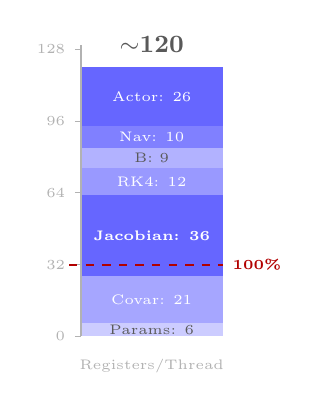
\begin{tikzpicture}[scale=0.75]
    % Stacked bar chart with unified blue colors
    \def\barwidth{2.4cm}
    \def\unit{0.038}

    % Draw stacked segments (bottom to top) - blue gradient
    \fill[blue!20] (0,0) rectangle (\barwidth, 6*\unit);
    \node[font=\tiny, text=gray!70!black] at (1.2, 3*\unit) {Params: 6};

    \fill[blue!35] (0,6*\unit) rectangle (\barwidth, 27*\unit);
    \node[font=\tiny, white] at (1.2, 16.5*\unit) {Covar: 21};

    \fill[blue!60] (0,27*\unit) rectangle (\barwidth, 63*\unit);
    \node[font=\tiny\bfseries, white] at (1.2, 45*\unit) {Jacobian: 36};

    \fill[blue!40] (0,63*\unit) rectangle (\barwidth, 75*\unit);
    \node[font=\tiny, white] at (1.2, 69*\unit) {RK4: 12};

    \fill[blue!30] (0,75*\unit) rectangle (\barwidth, 84*\unit);
    \node[font=\tiny, text=gray!70!black] at (1.2, 79.5*\unit) {B: 9};

    \fill[blue!50] (0,84*\unit) rectangle (\barwidth, 94*\unit);
    \node[font=\tiny, white] at (1.2, 89*\unit) {Nav: 10};

    \fill[blue!60] (0,94*\unit) rectangle (\barwidth, 120*\unit);
    \node[font=\tiny, white] at (1.2, 107*\unit) {Actor: 26};

    % Y-axis
    \draw[gray!60, thick] (0,0) -- (0, 130*\unit);
    \foreach \y/\lab in {0/0, 32/32, 64/64, 96/96, 128/128} {
        \draw[gray!60] (-0.1, \y*\unit) -- (0, \y*\unit);
        \node[left, font=\tiny, text=gray!60] at (-0.1, \y*\unit) {\lab};
    }

    % 100% occupancy line
    \draw[red!70!black, thick, dashed] (-0.2, 32*\unit) -- (\barwidth+0.4, 32*\unit);
    \node[right, font=\tiny\bfseries, text=red!70!black] at (\barwidth+0.15, 32*\unit) {100\%};

    % Total label
    \node[above, font=\small\bfseries, text=gray!70!black] at (1.2, 122*\unit) {$\sim$120};

    % X-axis label
    \node[font=\tiny, text=gray!60] at (1.2, -0.5) {Registers/Thread};
\end{tikzpicture}

\vspace{0.2em}
\begin{alertblock}{Key Insight}
    \textcolor{blue!70!black}{\textbf{Jacobian}} only needed for MBF smoother!
\end{alertblock}
\end{columns}
\end{frame}

\begin{frame}{Opportunity: Conditional Jacobian}
\begin{columns}
\column{0.55\textwidth}
\textbf{When is Jacobian Needed?}
\begin{itemize}
    \item Multi-Branch Fit (MBF) smoother requires accumulated Jacobian
    \item Used for backward smoothing pass
    \item When MBF disabled: Jacobian computed but \textbf{never used}
\end{itemize}

\vspace{0.5em}
\textbf{Current Behavior (parameter\_transporter)}
\begin{enumerate}
    \item Compute full 6$\times$6 Jacobian at each surface
    \item Multiply: $J_{acc} = J_{new} \times J_{acc}$ (6$\times$6 $\times$ 6$\times$6)
    \item Store accumulated Jacobian to global memory
    \item \textcolor{red}{Wasted work when MBF=false!}
\end{enumerate}

\column{0.45\textwidth}
\centering
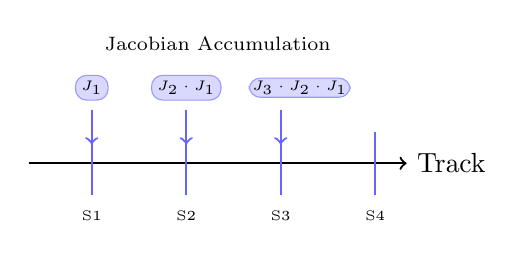
\begin{tikzpicture}[scale=0.8]
    % Track with surfaces
    \draw[thick,->] (0,0) -- (6,0) node[right] {Track};

    % Surfaces
    \foreach \x/\label in {1/S1, 2.5/S2, 4/S3, 5.5/S4} {
        \draw[thick,blue!60] (\x,-0.5) -- (\x,0.5);
        \node[below] at (\x,-0.6) {\tiny \label};
    }

    % Jacobian accumulation - spread out more
    \node[draw=blue!40, fill=blue!15, rounded corners, font=\tiny, inner sep=2pt] at (1,1.2) {$J_1$};
    \node[draw=blue!40, fill=blue!15, rounded corners, font=\tiny, inner sep=2pt] at (2.5,1.2) {$J_2 \cdot J_1$};
    \node[draw=blue!40, fill=blue!15, rounded corners, font=\tiny, inner sep=1pt] at (4.3,1.2) {$J_3 \cdot J_2 \cdot J_1$};

    % Arrow indicating accumulation
    \draw[->,thick,blue!60] (1,0.85) -- (1,0.3);
    \draw[->,thick,blue!60] (2.5,0.85) -- (2.5,0.3);
    \draw[->,thick,blue!60] (4,0.85) -- (4,0.3);

    % Label
    \node[font=\scriptsize] at (3,1.9) {Jacobian Accumulation};
\end{tikzpicture}

\vspace{0.5em}
\begin{block}{Savings per Surface}
\begin{itemize}
    \item $\sim$216 FLOPs (matrix mult)
    \item $\sim$288 bytes memory I/O
\end{itemize}
\end{block}
\end{columns}
\end{frame}

%==============================================================================%
\section{Implementation}
%==============================================================================%

\begin{frame}{Solution: Two Actor Chains}
\begin{columns}
\column{0.55\textwidth}
{\scriptsize\textbf{Original: \texttt{ckf\_actor\_chain\_t}}}
\begin{enumerate}\itemsep-2pt\parskip0pt\topsep0pt
    \item {\tiny\texttt{pathlimit\_aborter}}
    \item {\tiny\textcolor{gray!70}{\texttt{parameter\_transporter}} $\leftarrow$ Jacobian ptr}
    \item {\tiny\texttt{interaction\_register}}
    \item {\tiny\texttt{ckf\_interactor}}
    \item {\tiny\texttt{parameter\_resetter}}
    \item {\tiny\texttt{momentum\_aborter}}
    \item {\tiny\texttt{ckf\_aborter}}
\end{enumerate}

{\scriptsize\textbf{New: \texttt{ckf\_actor\_chain\_no\_mbf\_t}}}
\begin{enumerate}\itemsep-2pt\parskip0pt\topsep0pt
    \item {\tiny\texttt{pathlimit\_aborter}}
    \item {\tiny\textcolor{green!50!black}{\texttt{bound\_updater}} $\leftarrow$ \textbf{Empty state!}}
    \item {\tiny\texttt{interaction\_register}}
    \item {\tiny\texttt{ckf\_interactor}}
    \item {\tiny\texttt{parameter\_resetter}}
    \item {\tiny\texttt{momentum\_aborter}}
    \item {\tiny\texttt{ckf\_aborter}}
\end{enumerate}

\column{0.45\textwidth}
\centering
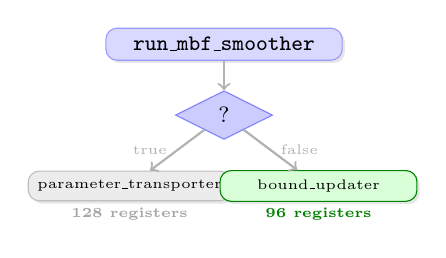
\begin{tikzpicture}[scale=0.6]
    % Runtime dispatch
    \node[draw=blue!40, rounded corners, fill=blue!15, minimum width=3cm, drop shadow={shadow xshift=1pt, shadow yshift=-1pt, opacity=0.2}] (config) at (0,3) {\footnotesize \texttt{run\_mbf\_smoother}};

    % Decision diamond
    \node[draw=blue!50, diamond, fill=blue!20, aspect=2] (decision) at (0,1.5) {\footnotesize ?};

    % Two paths
    \node[draw=gray!50, rounded corners, fill=gray!15, minimum width=2.5cm, font=\tiny, drop shadow={shadow xshift=1pt, shadow yshift=-1pt, opacity=0.2}] (mbf_on) at (-2,0) {parameter\_transporter};
    \node[draw=green!50!black, rounded corners, fill=green!15, minimum width=2.5cm, font=\tiny, drop shadow={shadow xshift=1pt, shadow yshift=-1pt, opacity=0.2}] (mbf_off) at (2,0) {bound\_updater};

    % Arrows
    \draw[->,thick,gray!60] (config) -- (decision);
    \draw[->,thick,gray!60] (decision) -- node[left,font=\tiny] {true} (mbf_on);
    \draw[->,thick,gray!60] (decision) -- node[right,font=\tiny] {false} (mbf_off);

    % Labels
    \node[font=\tiny\bfseries,text=gray!70] at (-2,-0.6) {128 registers};
    \node[font=\tiny\bfseries,text=green!50!black] at (2,-0.6) {96 registers};
\end{tikzpicture}

\begin{block}{Compile-Time Dispatch}
    {\scriptsize\texttt{if constexpr} selects actor chain based on propagator type}
\end{block}
\end{columns}
\end{frame}

\begin{frame}{Key Code: Actor State Comparison}
\begin{columns}
\column{0.5\textwidth}
\centering
\textbf{parameter\_transporter}\\{\scriptsize (detray - original)}

\vspace{0.2em}
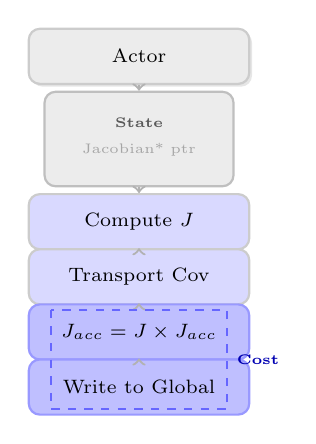
\begin{tikzpicture}[scale=0.7,
    box/.style={draw=gray!40, rounded corners, minimum width=2.8cm, minimum height=0.7cm, font=\scriptsize, line width=0.8pt},
    statebox/.style={draw=gray!50, rounded corners, fill=gray!15, minimum width=2.4cm, minimum height=1.2cm, font=\tiny, line width=0.8pt},
    flowarrow/.style={->, thick, gray!60}
]
    % Actor box
    \node[box, fill=gray!15, drop shadow={shadow xshift=1pt, shadow yshift=-1pt, opacity=0.2}] (actor) at (0,2.5) {Actor};

    % State box with Jacobian pointer
    \node[statebox] (state) at (0,1) {};
    \node[font=\tiny\bfseries, text=gray!70!black] at (0,1.3) {State};
    \node[font=\tiny, text=gray!70] at (0,0.8) {Jacobian* ptr};

    % Workflow
    \node[box, fill=blue!15] (compute) at (0,-0.5) {Compute $J$};
    \node[box, fill=blue!15] (transport) at (0,-1.5) {Transport Cov};
    \node[box, fill=blue!25, draw=blue!40] (aggregate) at (0,-2.5) {$J_{acc} = J \times J_{acc}$};
    \node[box, fill=blue!25, draw=blue!40] (write) at (0,-3.5) {Write to Global};

    % Arrows
    \draw[flowarrow] (actor) -- (state);
    \draw[flowarrow] (state) -- (compute);
    \draw[flowarrow] (compute) -- (transport);
    \draw[flowarrow] (transport) -- (aggregate);
    \draw[flowarrow] (aggregate) -- (write);

    % Highlight expensive ops
    \draw[blue!60, thick, dashed] (-1.6,-2.1) rectangle (1.6,-3.9);
    \node[font=\tiny\bfseries, text=blue!70!black, right] at (1.6,-3) {Cost};
\end{tikzpicture}

\column{0.5\textwidth}
\centering
\textbf{bound\_updater}\\{\scriptsize (traccc - optimized)}

\vspace{0.2em}
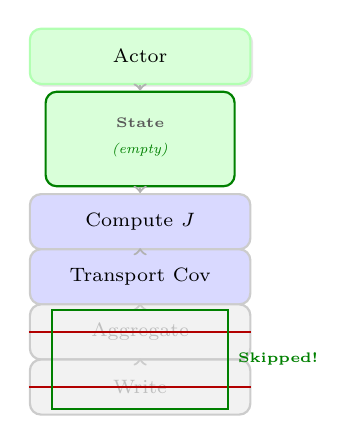
\begin{tikzpicture}[scale=0.7,
    box/.style={draw=gray!40, rounded corners, minimum width=2.8cm, minimum height=0.7cm, font=\scriptsize, line width=0.8pt},
    statebox/.style={draw=green!50!black, rounded corners, fill=green!15, minimum width=2.4cm, minimum height=1.2cm, font=\tiny, line width=0.8pt},
    flowarrow/.style={->, thick, gray!60}
]
    % Actor box
    \node[box, fill=green!15, draw=green!30, drop shadow={shadow xshift=1pt, shadow yshift=-1pt, opacity=0.2}] (actor) at (0,2.5) {Actor};

    % Empty state box
    \node[statebox] (state) at (0,1) {};
    \node[font=\tiny\bfseries, text=gray!70!black] at (0,1.3) {State};
    \node[font=\tiny, text=green!50!black] at (0,0.8) {\textit{(empty)}};

    % Workflow
    \node[box, fill=blue!15] (compute) at (0,-0.5) {Compute $J$};
    \node[box, fill=blue!15] (transport) at (0,-1.5) {Transport Cov};
    \node[box, fill=gray!10, draw=gray!40, text=gray!50] (skip1) at (0,-2.5) {Aggregate};
    \draw[red!70!black, thick] (skip1.west) -- (skip1.east);
    \node[box, fill=gray!10, draw=gray!40, text=gray!50] (skip2) at (0,-3.5) {Write};
    \draw[red!70!black, thick] (skip2.west) -- (skip2.east);

    % Arrows
    \draw[flowarrow] (actor) -- (state);
    \draw[flowarrow] (state) -- (compute);
    \draw[flowarrow] (compute) -- (transport);
    \draw[->, thick, gray!40, dashed] (transport) -- (skip1);
    \draw[->, thick, gray!40, dashed] (skip1) -- (skip2);

    % Highlight skipped
    \draw[green!50!black, thick] (-1.6,-2.1) rectangle (1.6,-3.9);
    \node[font=\tiny\bfseries, text=green!50!black, right] at (1.6,-3) {Skipped!};
\end{tikzpicture}
\end{columns}

\vspace{0.2em}
\begin{alertblock}{Key Difference}
    Empty state $\rightarrow$ \textbf{skip 6$\times$6 matrix mult \& global memory write}
\end{alertblock}
\end{frame}

\begin{frame}{Kernel Dispatch Logic}
\vspace{-0.5em}
\begin{center}
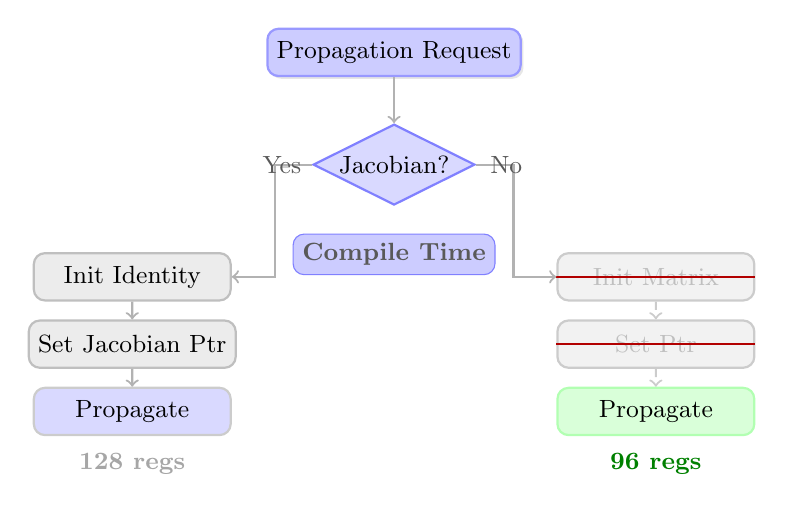
\begin{tikzpicture}[scale=0.95,
    decision/.style={diamond, draw=blue!50, fill=blue!15, minimum width=2cm, minimum height=1cm, aspect=2, font=\small, inner sep=1pt, line width=0.8pt},
    process/.style={draw=gray!40, rounded corners, fill=blue!15, minimum width=2.5cm, minimum height=0.6cm, font=\small, line width=0.8pt},
    skipbox/.style={draw=gray!40, rounded corners, fill=gray!10, minimum width=2.5cm, minimum height=0.6cm, font=\small, text=gray!50, line width=0.8pt},
    myarrow/.style={->, thick, gray!60},
    tinylabel/.style={font=\small, text=gray!70!black}
]
    % Start
    \node[process, fill=blue!20, draw=blue!40, drop shadow={shadow xshift=1pt, shadow yshift=-1pt, opacity=0.2}] (start) at (0,2.5) {Propagation Request};

    % Decision diamond
    \node[decision] (check) at (0,1) {Jacobian?};

    % Yes branch (left)
    \node[process, fill=gray!15, draw=gray!50] (init1) at (-3.5,-0.5) {Init Identity};
    \node[process, fill=gray!15, draw=gray!50] (init2) at (-3.5,-1.4) {Set Jacobian Ptr};
    \node[process] (prop1) at (-3.5,-2.3) {Propagate};

    % No branch (right) - crossed out text
    \node[skipbox] (skip1) at (3.5,-0.5) {Init Matrix};
    \draw[red!70!black, thick] (skip1.west) -- (skip1.east);
    \node[skipbox] (skip2) at (3.5,-1.4) {Set Ptr};
    \draw[red!70!black, thick] (skip2.west) -- (skip2.east);
    \node[process, fill=green!15, draw=green!30] (prop2) at (3.5,-2.3) {Propagate};

    % Arrows
    \draw[myarrow] (start) -- (check);
    \draw[myarrow] (check.west) -- ++(-0.5,0) |- (init1.east);
    \draw[myarrow] (check.east) -- ++(0.5,0) |- (skip1.west);
    \draw[myarrow] (init1) -- (init2);
    \draw[myarrow] (init2) -- (prop1);
    \draw[->, thick, gray!40, dashed] (skip1) -- (skip2);
    \draw[->, thick, gray!40, dashed] (skip2) -- (prop2);

    % Branch labels
    \node[tinylabel] at (-1.5,1) {Yes};
    \node[tinylabel] at (1.5,1) {No};

    % Compile-time badge
    \node[draw=blue!50, rounded corners, fill=blue!20, font=\small\bfseries, text=gray!70!black] at (0,-0.2) {Compile Time};

    % Labels for branches
    \node[font=\small\bfseries, text=gray!70] at (-3.5,-3) {128 regs};
    \node[font=\small\bfseries, text=green!50!black] at (3.5,-3) {96 regs};
\end{tikzpicture}
\end{center}

\begin{block}{18 Kernel Specializations}
    3 detector types $\times$ 3 B-field configs $\times$ 2 MBF variants
\end{block}
\end{frame}

%==============================================================================%
\section{Results}
%==============================================================================%

\begin{frame}{Benchmark Results}
\vspace{-0.3em}
\begin{center}
% Performance Dashboard
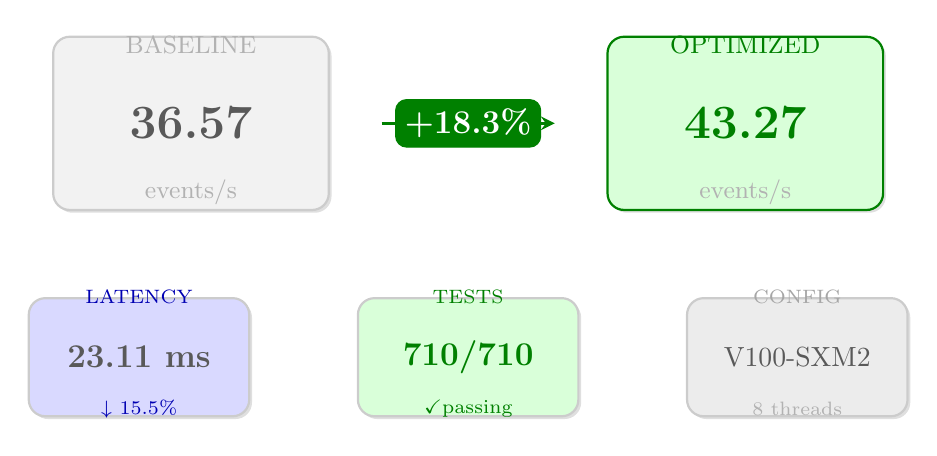
\begin{tikzpicture}[scale=1.1,
    scorecard/.style={draw=gray!40, rounded corners=6pt, minimum width=3.5cm, minimum height=2.2cm, font=\small, line width=0.8pt, drop shadow={shadow xshift=1pt, shadow yshift=-1pt, opacity=0.25}},
    arrow/.style={->, very thick, >=stealth}
]
    % Main throughput comparison
    \node[scorecard, fill=gray!10] (baseline) at (-3.2,1.5) {};
    \node[font=\small, text=gray!60] at (-3.2,2.4) {BASELINE};
    \node[font=\LARGE\bfseries, text=gray!70!black] at (-3.2,1.5) {36.57};
    \node[font=\small, text=gray!60] at (-3.2,0.7) {events/s};

    \node[scorecard, fill=green!15, draw=green!50!black] (opt) at (3.2,1.5) {};
    \node[font=\small, text=green!50!black] at (3.2,2.4) {OPTIMIZED};
    \node[font=\LARGE\bfseries, text=green!50!black] at (3.2,1.5) {43.27};
    \node[font=\small, text=gray!60] at (3.2,0.7) {events/s};

    % Arrow with improvement badge
    \draw[arrow, green!50!black] (-1,1.5) -- (1,1.5);
    \node[draw=green!50!black, rounded corners, fill=green!50!black, font=\large\bfseries, text=white] at (0,1.5) {+18.3\%};

    % Secondary metrics row
    \node[scorecard, fill=blue!15, minimum width=2.8cm, minimum height=1.5cm] (latency) at (-3.8,-1.2) {};
    \node[font=\scriptsize, text=blue!70!black] at (-3.8,-0.5) {LATENCY};
    \node[font=\large\bfseries, text=gray!70!black] at (-3.8,-1.2) {23.11 ms};
    \node[font=\scriptsize, text=blue!70!black] at (-3.8,-1.8) {$\downarrow$ 15.5\%};

    \node[scorecard, fill=green!15, minimum width=2.8cm, minimum height=1.5cm] (tests) at (0,-1.2) {};
    \node[font=\scriptsize, text=green!50!black] at (0,-0.5) {TESTS};
    \node[font=\large\bfseries, text=green!50!black] at (0,-1.2) {710/710};
    \node[font=\scriptsize, text=green!50!black] at (0,-1.8) {\checkmark passing};

    \node[scorecard, fill=gray!15, minimum width=2.8cm, minimum height=1.5cm] (config) at (3.8,-1.2) {};
    \node[font=\scriptsize, text=gray!70] at (3.8,-0.5) {CONFIG};
    \node[font=\normalsize, text=gray!70!black] at (3.8,-1.2) {V100-SXM2};
    \node[font=\scriptsize, text=gray!60] at (3.8,-1.8) {8 threads};

\end{tikzpicture}
\end{center}

\begin{columns}
\column{0.5\textwidth}
\centering
{\small\textit{Apples-to-apples: Both with MBF=false}}
\column{0.5\textwidth}
\centering
{\small Dataset: \texttt{ttbar\_mu200}}
\end{columns}
\end{frame}

\begin{frame}{Methodology: Isolating the True Improvement}
\begin{columns}[T]
\column{0.55\textwidth}
\textbf{The Problem}
\begin{itemize}\itemsep2pt
    \item Initial benchmark: \textbf{+11.67\%} (38.75 $\rightarrow$ 43.27)
    \item But \texttt{build\_tracks} improved by 86\%!
    \item Confounding variable: MBF default changed
\end{itemize}

\vspace{0.5em}
\textbf{The Solution}
\begin{itemize}\itemsep2pt
    \item Re-benchmark with controlled config
    \item Both baseline and optimization: MBF=false
    \item Isolated result: \textbf{+18.3\%} (36.57 $\rightarrow$ 43.27)
\end{itemize}

\column{0.45\textwidth}
\centering
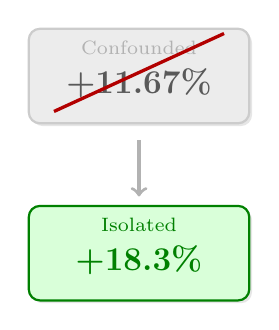
\begin{tikzpicture}[scale=0.9]
    % Confounded result (crossed out)
    \node[draw=gray!40, rounded corners, fill=gray!15, minimum width=2.8cm, minimum height=1.2cm, line width=0.8pt, drop shadow={shadow xshift=1pt, shadow yshift=-1pt, opacity=0.2}] at (0,2) {};
    \node[font=\scriptsize, text=gray!60] at (0,2.4) {Confounded};
    \node[font=\large\bfseries, text=gray!70!black] at (0,1.9) {+11.67\%};
    \draw[red!70!black, very thick] (-1.2,1.5) -- (1.2,2.6);

    % Arrow
    \draw[->, very thick, gray!60] (0,1.1) -- (0,0.3);

    % Isolated result
    \node[draw=green!50!black, rounded corners, fill=green!15, minimum width=2.8cm, minimum height=1.2cm, line width=0.8pt, drop shadow={shadow xshift=1pt, shadow yshift=-1pt, opacity=0.2}] at (0,-0.5) {};
    \node[font=\scriptsize, text=green!50!black] at (0,-0.1) {Isolated};
    \node[font=\large\bfseries, text=green!50!black] at (0,-0.6) {+18.3\%};
\end{tikzpicture}
\end{columns}

\vspace{0.3em}
\begin{alertblock}{Lesson Learned}
    Always control for configuration changes! The true optimization impact was \textbf{larger} than initially measured.
\end{alertblock}
\end{frame}

\begin{frame}{NCU Profiling: Key Metrics Dashboard}
\vspace{-0.3em}
{\small \textit{RTX 2080 Ti (sm\_75), ncu 2024.1.1}}
\begin{center}
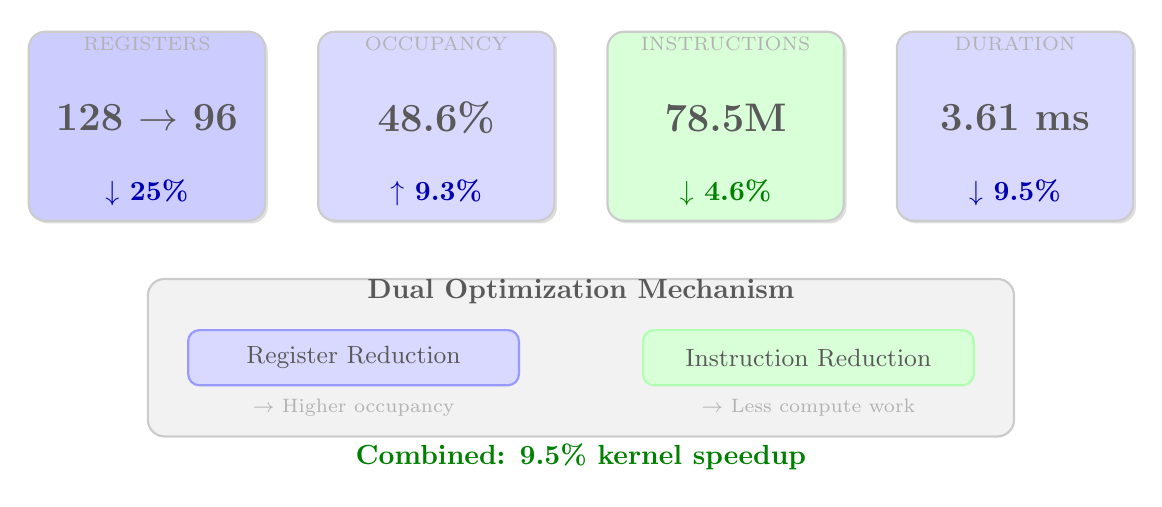
\begin{tikzpicture}[scale=1.05,
    card/.style={draw=gray!40, rounded corners=6pt, minimum width=3cm, minimum height=2.4cm, line width=0.8pt, drop shadow={shadow xshift=1pt, shadow yshift=-1pt, opacity=0.25}},
    biglabel/.style={font=\Large\bfseries},
    smalllabel/.style={font=\scriptsize, text=gray!60},
    change/.style={font=\normalsize\bfseries}
]
    % Top row - 4 key metrics
    % Registers
    \node[card, fill=blue!20] (reg) at (-5,1.5) {};
    \node[smalllabel] at (-5,2.5) {REGISTERS};
    \node[biglabel, text=gray!70!black] at (-5,1.6) {128 $\rightarrow$ 96};
    \node[change, text=blue!70!black] at (-5,0.7) {$\downarrow$ 25\%};

    % Occupancy
    \node[card, fill=blue!15] (occ) at (-1.5,1.5) {};
    \node[smalllabel] at (-1.5,2.5) {OCCUPANCY};
    \node[biglabel, text=gray!70!black] at (-1.5,1.6) {48.6\%};
    \node[change, text=blue!70!black] at (-1.5,0.7) {$\uparrow$ 9.3\%};

    % Instructions
    \node[card, fill=green!15] (inst) at (2,1.5) {};
    \node[smalllabel] at (2,2.5) {INSTRUCTIONS};
    \node[biglabel, text=gray!70!black] at (2,1.6) {78.5M};
    \node[change, text=green!50!black] at (2,0.7) {$\downarrow$ 4.6\%};

    % Duration
    \node[card, fill=blue!15] (dur) at (5.5,1.5) {};
    \node[smalllabel] at (5.5,2.5) {DURATION};
    \node[biglabel, text=gray!70!black] at (5.5,1.6) {3.61 ms};
    \node[change, text=blue!70!black] at (5.5,0.7) {$\downarrow$ 9.5\%};

    % Mechanism explanation below
    \node[draw=gray!40, rounded corners=6pt, fill=gray!10, minimum width=11cm, minimum height=2cm, line width=0.8pt] at (0.25,-1.3) {};
    \node[font=\normalsize\bfseries, text=gray!70!black] at (0.25,-0.5) {Dual Optimization Mechanism};

    % Left mechanism
    \node[draw=blue!40, rounded corners, fill=blue!15, minimum width=4.2cm, minimum height=0.7cm, font=\small, text=gray!70!black, line width=0.8pt] at (-2.5,-1.3) {Register Reduction};
    \node[font=\scriptsize, text=gray!60] at (-2.5,-1.9) {$\rightarrow$ Higher occupancy};

    % Right mechanism
    \node[draw=green!30, rounded corners, fill=green!15, minimum width=4.2cm, minimum height=0.7cm, font=\small, text=gray!70!black, line width=0.8pt] at (3,-1.3) {Instruction Reduction};
    \node[font=\scriptsize, text=gray!60] at (3,-1.9) {$\rightarrow$ Less compute work};

    % Combined result
    \node[font=\normalsize\bfseries, text=green!50!black] at (0.25,-2.5) {Combined: 9.5\% kernel speedup};

\end{tikzpicture}
\end{center}
\end{frame}

\begin{frame}{Architecture-Dependent Behavior}
\begin{center}
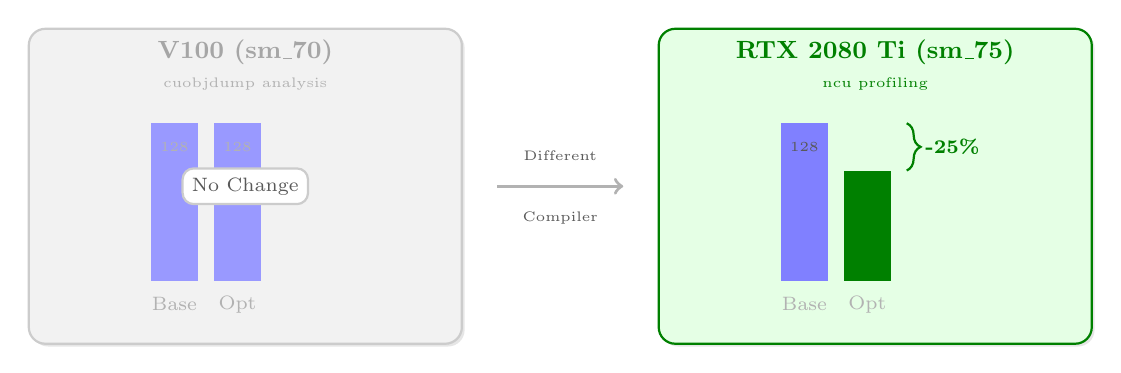
\begin{tikzpicture}[
    panel/.style={draw=gray!40, rounded corners=6pt, minimum width=5.5cm, minimum height=4cm, line width=0.8pt, drop shadow={shadow xshift=1pt, shadow yshift=-1pt, opacity=0.2}},
    barlabel/.style={font=\scriptsize, text=gray!60}
]
    % V100 Panel (left) - faded
    \node[panel, fill=gray!10] (v100) at (-4,0) {};
    \node[font=\small\bfseries, text=gray!70] at (-4,1.7) {V100 (sm\_70)};
    \node[font=\tiny, text=gray!60] at (-4,1.3) {cuobjdump analysis};

    % V100 bars - same height
    \fill[blue!40] (-5.2,-1.2) rectangle (-4.6,0.8);
    \fill[blue!40] (-4.4,-1.2) rectangle (-3.8,0.8);
    \node[barlabel] at (-4.9,-1.5) {Base};
    \node[barlabel] at (-4.1,-1.5) {Opt};
    \node[font=\tiny, text=gray!60] at (-4.9,0.5) {128};
    \node[font=\tiny, text=gray!60] at (-4.1,0.5) {128};

    % No change indicator
    \node[draw=gray!40, rounded corners, fill=white, font=\scriptsize, text=gray!70!black, line width=0.8pt] at (-4,0) {No Change};

    % RTX 2080 Ti Panel (right) - highlighted
    \node[panel, fill=green!10, draw=green!50!black] (rtx) at (4,0) {};
    \node[font=\small\bfseries, text=green!50!black] at (4,1.7) {RTX 2080 Ti (sm\_75)};
    \node[font=\tiny, text=green!50!black] at (4,1.3) {ncu profiling};

    % RTX bars - different heights
    \fill[blue!50] (2.8,-1.2) rectangle (3.4,0.8);
    \fill[green!50!black] (3.6,-1.2) rectangle (4.2,0.2);
    \node[barlabel] at (3.1,-1.5) {Base};
    \node[barlabel] at (3.9,-1.5) {Opt};
    \node[font=\tiny, text=gray!70!black] at (3.1,0.5) {128};
    \node[font=\tiny\bfseries, text=green!50!black] at (3.9,-0.1) {96};

    % Bracket showing reduction
    \draw[thick, green!50!black, decorate, decoration={brace, amplitude=5pt}]
        (4.4,0.8) -- (4.4,0.2) node[midway, right, font=\scriptsize\bfseries, xshift=3pt, text=green!50!black] {-25\%};

    % Arrow between panels
    \draw[->, very thick, gray!60] (-0.8,0) -- (0.8,0);
    \node[font=\tiny, above, text=gray!70!black] at (0,0.2) {Different};
    \node[font=\tiny, below, text=gray!70!black] at (0,-0.2) {Compiler};

\end{tikzpicture}
\end{center}

\vspace{0.2em}
\begin{alertblock}{Key Insight}
    \textbf{Always profile on target hardware!} The same code compiles to different register counts on different architectures.
\end{alertblock}
\end{frame}

\begin{frame}{Optimization Mechanism Summary}
\begin{center}
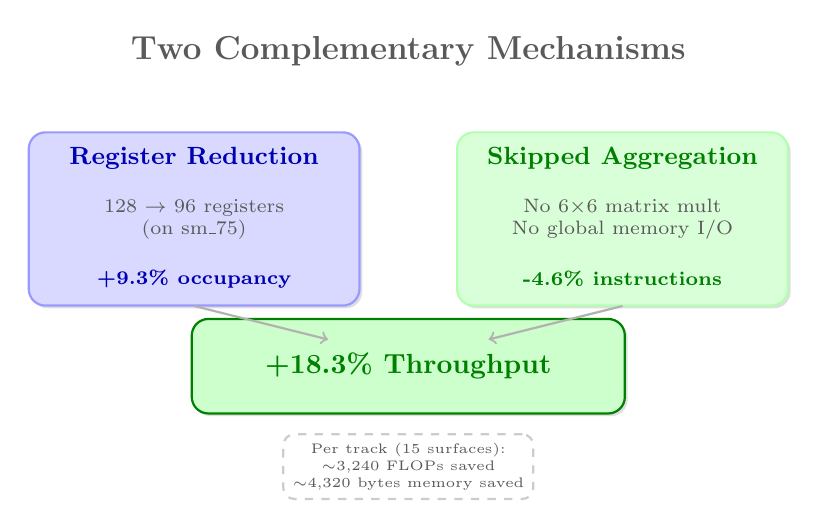
\begin{tikzpicture}[scale=0.85]
    % Title
    \node[font=\large\bfseries, text=gray!70!black] at (0,4) {Two Complementary Mechanisms};

    % Mechanism 1 - Register Reduction
    \node[draw=blue!40, rounded corners=6pt, fill=blue!15, minimum width=4.2cm, minimum height=2.2cm, line width=0.8pt, drop shadow={shadow xshift=1pt, shadow yshift=-1pt, opacity=0.25}] (mech1) at (-3.2,1.5) {};
    \node[font=\small\bfseries, text=blue!70!black] at (-3.2,2.4) {Register Reduction};
    \node[font=\scriptsize, align=center, text=gray!70!black] at (-3.2,1.5) {128 $\rightarrow$ 96 registers\\(on sm\_75)};
    \node[font=\scriptsize\bfseries, text=blue!70!black] at (-3.2,0.6) {+9.3\% occupancy};

    % Mechanism 2 - Skipped Aggregation
    \node[draw=green!30, rounded corners=6pt, fill=green!15, minimum width=4.2cm, minimum height=2.2cm, line width=0.8pt, drop shadow={shadow xshift=1pt, shadow yshift=-1pt, opacity=0.25}] (mech2) at (3.2,1.5) {};
    \node[font=\small\bfseries, text=green!50!black] at (3.2,2.4) {Skipped Aggregation};
    \node[font=\scriptsize, align=center, text=gray!70!black] at (3.2,1.5) {No 6$\times$6 matrix mult\\No global memory I/O};
    \node[font=\scriptsize\bfseries, text=green!50!black] at (3.2,0.6) {-4.6\% instructions};

    % Combined effect
    \node[draw=green!50!black, rounded corners=6pt, fill=green!20, minimum width=5.5cm, minimum height=1.2cm, line width=0.8pt, drop shadow={shadow xshift=1pt, shadow yshift=-1pt, opacity=0.25}] (result) at (0,-0.7) {};
    \node[font=\normalsize\bfseries, text=green!50!black] at (0,-0.7) {+18.3\% Throughput};

    % Arrows
    \draw[->, thick, gray!60] (-3.2,0.2) -- (-1.2,-0.3);
    \draw[->, thick, gray!60] (3.2,0.2) -- (1.2,-0.3);

    % Per-track savings
    \node[draw=gray!40, dashed, rounded corners=4pt, fill=white, font=\tiny, align=center, text=gray!70!black, line width=0.8pt] at (0,-2.2) {
        Per track (15 surfaces):\\
        $\sim$3,240 FLOPs saved\\
        $\sim$4,320 bytes memory saved
    };
\end{tikzpicture}
\end{center}
\end{frame}

%==============================================================================%
\section{Lessons Learned}
%==============================================================================%

\begin{frame}{Key Takeaways: Paper Analysis vs Real Hardware}
\begin{center}
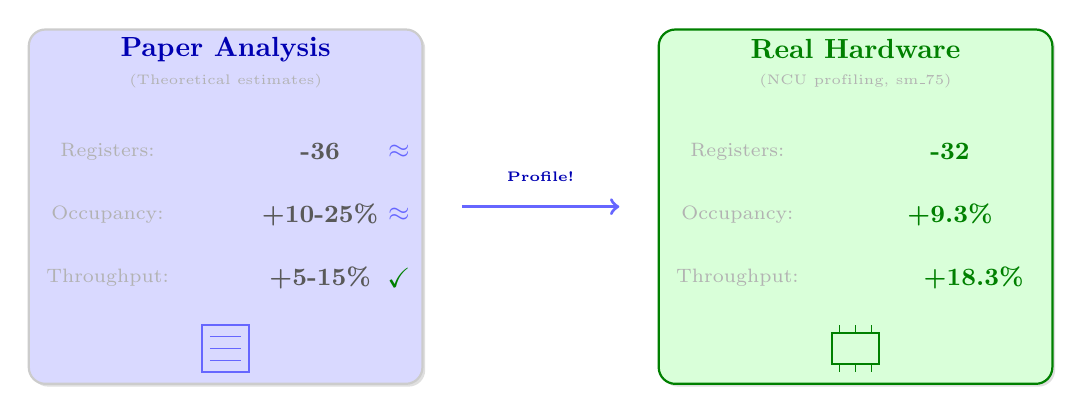
\begin{tikzpicture}[
    panel/.style={draw=gray!40, rounded corners=6pt, minimum width=5cm, minimum height=4.5cm, line width=0.8pt, drop shadow={shadow xshift=1pt, shadow yshift=-1pt, opacity=0.25}},
    metric/.style={font=\scriptsize},
    value/.style={font=\small\bfseries}
]
    % Paper Analysis Panel (left)
    \node[panel, fill=blue!15] (paper) at (-4,0.5) {};
    \node[font=\normalsize\bfseries, text=blue!70!black] at (-4,2.5) {Paper Analysis};
    \node[font=\tiny, text=gray!60] at (-4,2.1) {(Theoretical estimates)};

    % Paper metrics
    \node[metric, text=gray!60] at (-5.5,1.2) {Registers:};
    \node[value, text=gray!70!black] at (-2.8,1.2) {-36};
    \node[metric, text=gray!60] at (-5.5,0.4) {Occupancy:};
    \node[value, text=gray!70!black] at (-2.8,0.4) {+10-25\%};
    \node[metric, text=gray!60] at (-5.5,-0.4) {Throughput:};
    \node[value, text=gray!70!black] at (-2.8,-0.4) {+5-15\%};

    % Document icon (simple rectangle)
    \draw[blue!60, thick] (-4.3,-1.6) rectangle (-3.7,-1);
    \draw[blue!60] (-4.2,-1.15) -- (-3.8,-1.15);
    \draw[blue!60] (-4.2,-1.3) -- (-3.8,-1.3);
    \draw[blue!60] (-4.2,-1.45) -- (-3.8,-1.45);

    % Real Hardware Panel (right)
    \node[panel, fill=green!15, draw=green!50!black] (hw) at (4,0.5) {};
    \node[font=\normalsize\bfseries, text=green!50!black] at (4,2.5) {Real Hardware};
    \node[font=\tiny, text=gray!60] at (4,2.1) {(NCU profiling, sm\_75)};

    % Hardware metrics
    \node[metric, text=gray!60] at (2.5,1.2) {Registers:};
    \node[value, text=green!50!black] at (5.2,1.2) {-32};
    \node[metric, text=gray!60] at (2.5,0.4) {Occupancy:};
    \node[value, text=green!50!black] at (5.2,0.4) {+9.3\%};
    \node[metric, text=gray!60] at (2.5,-0.4) {Throughput:};
    \node[value, text=green!50!black] at (5.5,-0.4) {\textbf{+18.3\%}};

    % GPU icon (simple chip)
    \draw[green!50!black, thick] (3.7,-1.5) rectangle (4.3,-1.1);
    \foreach \x in {3.8,4,4.2} {
        \draw[green!50!black] (\x,-1.5) -- (\x,-1.6);
        \draw[green!50!black] (\x,-1.1) -- (\x,-1);
    }

    % Arrow between panels
    \draw[->, very thick, blue!60] (-1,0.5) -- (1,0.5);
    \node[font=\tiny\bfseries, text=blue!70!black, above] at (0,0.7) {Profile!};

    % Checkmarks/X marks
    \node[text=blue!60] at (-1.8,1.2) {$\approx$};
    \node[text=blue!60] at (-1.8,0.4) {$\approx$};
    \node[text=green!50!black] at (-1.8,-0.4) {\checkmark};

\end{tikzpicture}
\end{center}

\vspace{0.2em}
\begin{alertblock}{Important Caveat}
    Optimization only works when \textbf{MBF smoother is disabled}. Trade-off: No backward smoothing.
\end{alertblock}
\end{frame}

%==============================================================================%
\section{Conclusion}
%==============================================================================%

\begin{frame}{Summary}
\begin{columns}
\column{0.5\textwidth}
\textbf{Achievements}
\begin{itemize}\itemsep0pt
    \item \textbf{+18.3\%} throughput improvement
    \item \textbf{-25\%} register usage (on sm\_75)
    \item \textbf{+9.3\%} achieved occupancy
    \item \textbf{710/710} tests passing
\end{itemize}

\vspace{0.2em}
\textbf{Implementation}
\begin{itemize}\itemsep0pt
    \item New \texttt{bound\_updater} actor
    \item Two actor chain variants
    \item 18 kernel specializations
    \item Compile-time dispatch
\end{itemize}

\column{0.5\textwidth}
\textbf{Mechanism}
\begin{itemize}\itemsep0pt
    \item Skip 6$\times$6 matrix multiplication
    \item Reduce global memory traffic
    \item Architecture-dependent register savings
\end{itemize}

\vspace{0.2em}
\textbf{Key Files}
\begin{itemize}\itemsep0pt
    \item {\scriptsize\texttt{bound\_updater.hpp}}
    \item {\scriptsize\texttt{combinatorial\_kalman\_filter\_types.hpp}}
    \item {\scriptsize\texttt{propagate\_to\_next\_surface.ipp}}
\end{itemize}
\end{columns}

\vspace{0.1em}
\begin{block}{Conclusion}
    Conditional Jacobian Aggregation provides \textbf{+18.3\% throughput} through dual mechanism: register reduction (architecture-dependent) and skipped matrix operations (universal).
\end{block}
\end{frame}

\begin{frame}{Questions?}
\begin{center}
\vspace{1em}

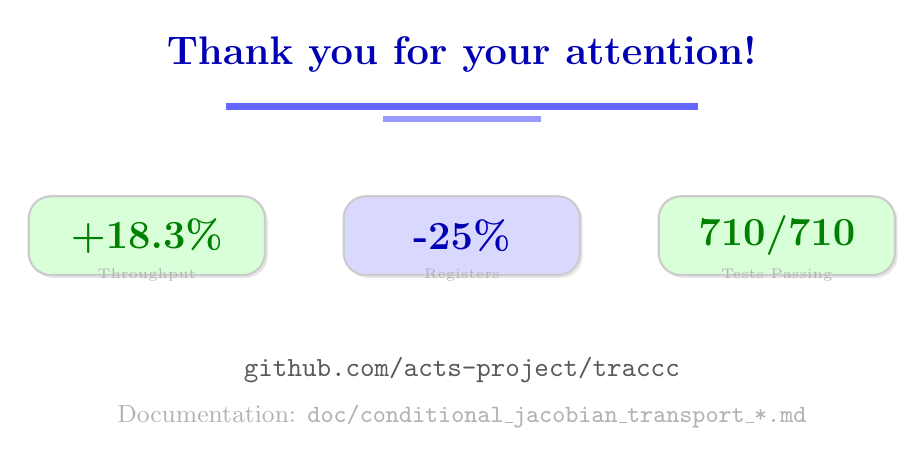
\begin{tikzpicture}
    % Main thank you message
    \node[font=\Large\bfseries, text=blue!70!black] at (0,2) {Thank you for your attention!};

    % Decorative line
    \fill[blue!60] (-3,1.3) rectangle (3,1.38);
    \fill[blue!40] (-1,1.15) rectangle (1,1.22);

    % Key results summary
    \node[draw=gray!40, rounded corners=8pt, fill=green!15, minimum width=3cm, minimum height=1cm, line width=0.8pt, drop shadow={shadow xshift=1pt, shadow yshift=-1pt, opacity=0.2}] at (-4,-0.3) {};
    \node[font=\Large\bfseries, text=green!50!black] at (-4,-0.3) {+18.3\%};
    \node[font=\tiny, text=gray!60] at (-4,-0.8) {Throughput};

    \node[draw=gray!40, rounded corners=8pt, fill=blue!15, minimum width=3cm, minimum height=1cm, line width=0.8pt, drop shadow={shadow xshift=1pt, shadow yshift=-1pt, opacity=0.2}] at (0,-0.3) {};
    \node[font=\Large\bfseries, text=blue!70!black] at (0,-0.3) {-25\%};
    \node[font=\tiny, text=gray!60] at (0,-0.8) {Registers};

    \node[draw=gray!40, rounded corners=8pt, fill=green!15, minimum width=3cm, minimum height=1cm, line width=0.8pt, drop shadow={shadow xshift=1pt, shadow yshift=-1pt, opacity=0.2}] at (4,-0.3) {};
    \node[font=\Large\bfseries, text=green!50!black] at (4,-0.3) {710/710};
    \node[font=\tiny, text=gray!60] at (4,-0.8) {Tests Passing};

    % Links
    \node[font=\normalsize, text=gray!70!black] at (0,-2) {\texttt{github.com/acts-project/traccc}};
    \node[font=\small, text=gray!60] at (0,-2.6) {Documentation: \texttt{doc/conditional\_jacobian\_transport\_*.md}};
\end{tikzpicture}

\end{center}
\end{frame}

%==============================================================================%
% BACKUP SLIDES
%==============================================================================%
\appendix
\newcounter{finalframe}
\setcounter{finalframe}{\value{framenumber}}

\begin{frame}{Backup: Anticipated Questions (1/2)}
\textbf{Q1: Why does Jacobian computation still happen?}
\begin{itemize}
    \item \texttt{get\_full\_jacobian()} is needed for covariance transport
    \item We skip the \textit{aggregation}, not the computation
    \item Future work: skip computation entirely when not needed
\end{itemize}

\vspace{0.5em}
\textbf{Q2: Why not runtime dispatch instead of compile-time?}
\begin{itemize}
    \item \texttt{if constexpr} allows dead code elimination
    \item Runtime \texttt{if} would still allocate registers for Jacobian pointer
    \item Compile-time dispatch enables different kernel specializations
\end{itemize}

\vspace{0.5em}
\textbf{Q3: What is MBF smoother and when is it needed?}
\begin{itemize}
    \item Multi-Branch Fit smoother: backward pass to improve track parameters
    \item Needed for high-precision physics measurements
    \item Can be disabled for real-time trigger applications
\end{itemize}
\end{frame}

\begin{frame}{Backup: Anticipated Questions (2/2)}
\textbf{Q4: Why different results on sm\_70 vs sm\_75?}
\begin{itemize}
    \item CUDA compiler makes architecture-specific optimizations
    \item Different instruction sets (sm\_75 has tensor cores)
    \item Register allocation heuristics vary by architecture
    \item Always profile on production hardware
\end{itemize}

\vspace{0.5em}
\textbf{Q5: What about other register-heavy kernels?}
\begin{itemize}
    \item \texttt{fit\_forward}: 168 registers
    \item \texttt{fit\_backward}: 168 registers
    \item Similar conditional optimization could apply
    \item Future work opportunity
\end{itemize}

\vspace{0.5em}
\textbf{Q6: How does this compare to other optimizations?}
\begin{itemize}
    \item Multi-event batching: +93\% throughput
    \item Conditional Jacobian: +18.3\% throughput
    \item Complementary optimizations, can be combined
\end{itemize}
\end{frame}

\begin{frame}{Backup: Detailed NCU Metrics}
\textbf{Full Profiling Data (RTX 2080 Ti, sm\_75, ncu 2024.1.1)}

\begin{columns}
\column{0.5\textwidth}
\begin{table}
    \tiny
    \begin{tabular}{lccc}
        \toprule
        \textbf{Metric} & \textbf{Base} & \textbf{Opt} & \textbf{$\Delta$} \\
        \midrule
        \multicolumn{4}{l}{\textit{Occupancy}} \\
        Registers/thread & 128 & 96 & -25\% \\
        Block limit & 4 & 5 & +25\% \\
        Theor. occupancy & 50.0\% & 62.5\% & +12.5\% \\
        Achieved occupancy & 39.28\% & 48.62\% & +9.34\% \\
        \midrule
        \multicolumn{4}{l}{\textit{Compute}} \\
        Duration (ms) & 3.99 & 3.61 & -9.5\% \\
        Instructions (M) & 82.3 & 78.5 & -4.6\% \\
        IPC & 0.26 & 0.26 & 0\% \\
        \bottomrule
    \end{tabular}
\end{table}

\column{0.5\textwidth}
\begin{table}
    \tiny
    \begin{tabular}{lccc}
        \toprule
        \textbf{Metric} & \textbf{Base} & \textbf{Opt} & \textbf{$\Delta$} \\
        \midrule
        \multicolumn{4}{l}{\textit{Memory}} \\
        Mem throughput & 218 GB/s & 245 GB/s & +12\% \\
        DRAM throughput & 33.2\% & 37.7\% & +4.5\% \\
        L1 hit rate & 54.1\% & 46.3\% & -7.8\% \\
        L2 hit rate & 79.6\% & 76.6\% & -3.0\% \\
        \midrule
        \multicolumn{4}{l}{\textit{Scheduler}} \\
        No eligible (\%) & 93.24\% & 93.27\% & +0.03\% \\
        Active warps/sched & 3.23 & 4.03 & +0.80 \\
        Warp cycles/instr & 47.74 & 59.92 & \textcolor{red}{+25\%} \\
        \bottomrule
    \end{tabular}
\end{table}
\end{columns}

\vspace{0.3em}
\begin{block}{Bottleneck Analysis}
    Kernel remains \textbf{latency-bound}: 93\% of cycles have no eligible warps.
    Note: Warp cycles/instruction \textit{increased} despite speedup---fewer total instructions but each waits longer (more memory parallelism).
\end{block}
\end{frame}

\setcounter{framenumber}{\value{finalframe}}
\end{document}
